% Figure from MATH 591 notes, section 67. After the board (Lecture 24): the configuration ruled out in the uniqueness proof.
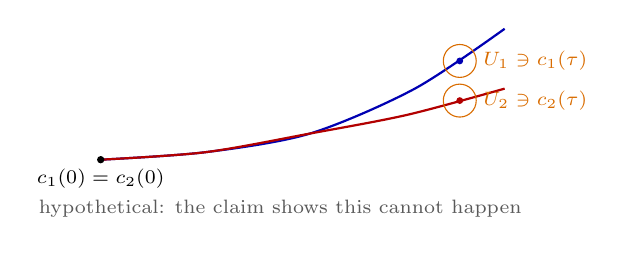
\begin{tikzpicture}[scale=0.95]
\draw[thick, blue!70!black] plot[smooth] coordinates {(-3,0) (-1.6,0.1) (-0.2,0.35) (1.2,0.95) (2.4,1.75)};
\draw[thick, red!70!black] plot[smooth] coordinates {(-3,0) (-1.6,0.1) (-0.2,0.35) (1.1,0.6) (2.4,0.95)};
\fill (-3,0) circle (1.4pt) node[below, font=\scriptsize] {$c_1(0) = c_2(0)$};
\fill[blue!70!black] (1.8,1.32) circle (1.3pt); \fill[red!70!black] (1.8,0.79) circle (1.3pt);
\draw[orange!85!black] (1.8,1.32) circle (0.22) node[right=5pt, font=\scriptsize] {$U_1 \ni c_1(\tau)$};
\draw[orange!85!black] (1.8,0.79) circle (0.22) node[right=5pt, font=\scriptsize] {$U_2 \ni c_2(\tau)$};
\node[font=\scriptsize, align=center, gray!70!black] at (-0.6,-0.65) {hypothetical: the claim shows this cannot happen};
\end{tikzpicture}
